\newpage
\section{Generator stability and System Analysis Assessment}
\renewcommand{\thesubsection}{\thesection.\alph{subsection}}
    \subsection{}
        \begin{figure}[tbh!]
            \centering
            \caption*{N.B. the diagram is not to scale and all angles are in degrees}
            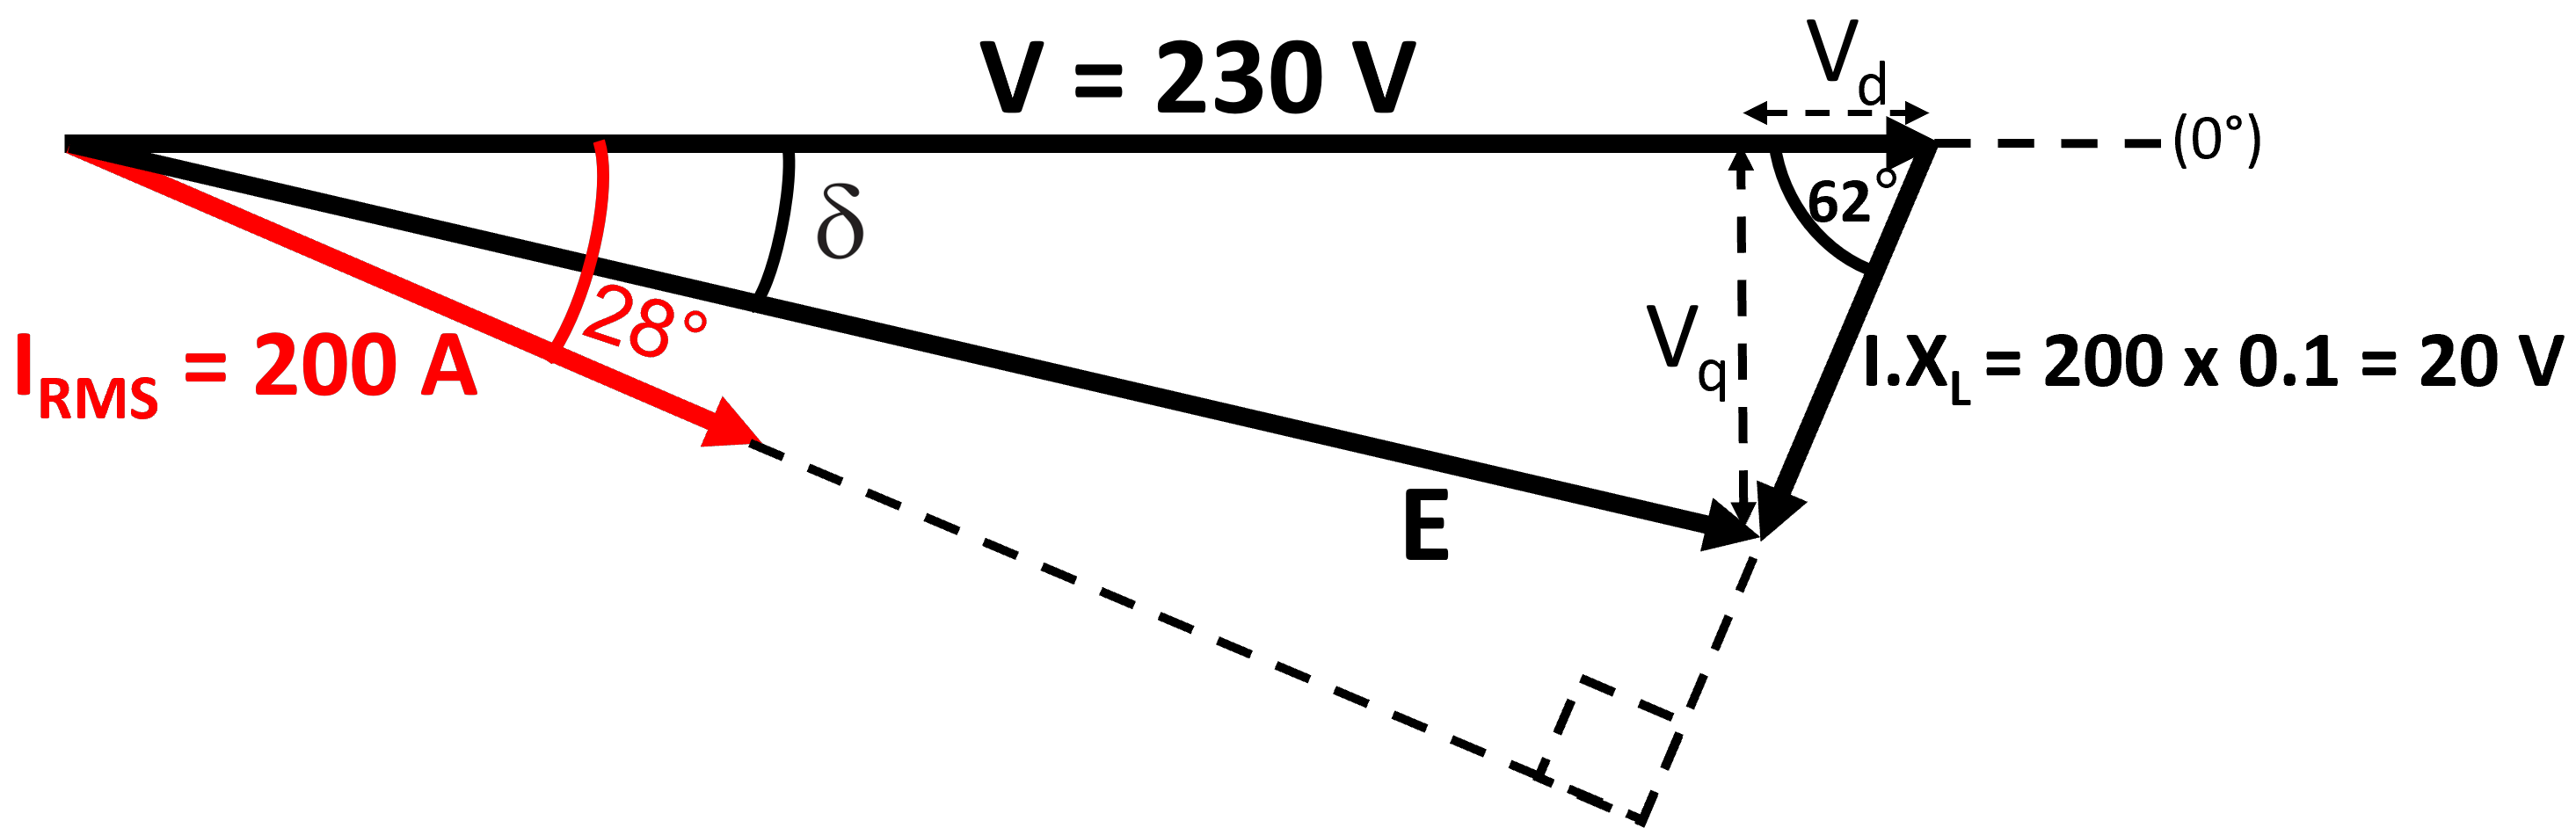
\includegraphics[width=\linewidth]{PEMDT Exam Report/img/Phasor Diagram.png}
            \caption{Phasor diagram for part (a)}
            \label{fig: phasor diagram}
        \end{figure}

        Assuming the motor's resistance is negligible and the machine is in a motoring state, the phasor diagram of the system is shown in Figure \ref{fig: phasor diagram}. This phasor diagram can be used to work out the magnitude (\(E\)) and phase (\(\delta\)) of the internal voltage of the motor as shown below:
        \begin{align}
            V_d = IX_L \cos(62) = 9.389 \text{V} && V_q = IX_L \sin(62) = 17.659 \text{V} \\
            \textbf{E} = \sqrt{\left(V - V_d\right)^2 + {V_{q}}^2} = \textbf{221.316} \text{\textbf{V}} && \delta = \tan^{-1}\left(\frac{V_q}{V - V_d}\right) = \textbf{4.577}^\textbf{o}
        \end{align}

    \subsection{}
        \begin{figure}[tbh!]
            \centering
            \caption*{N.B. all angles are in radians in this figure and question}
            \begin{subfigure}{0.49\textwidth}
                \centering
                 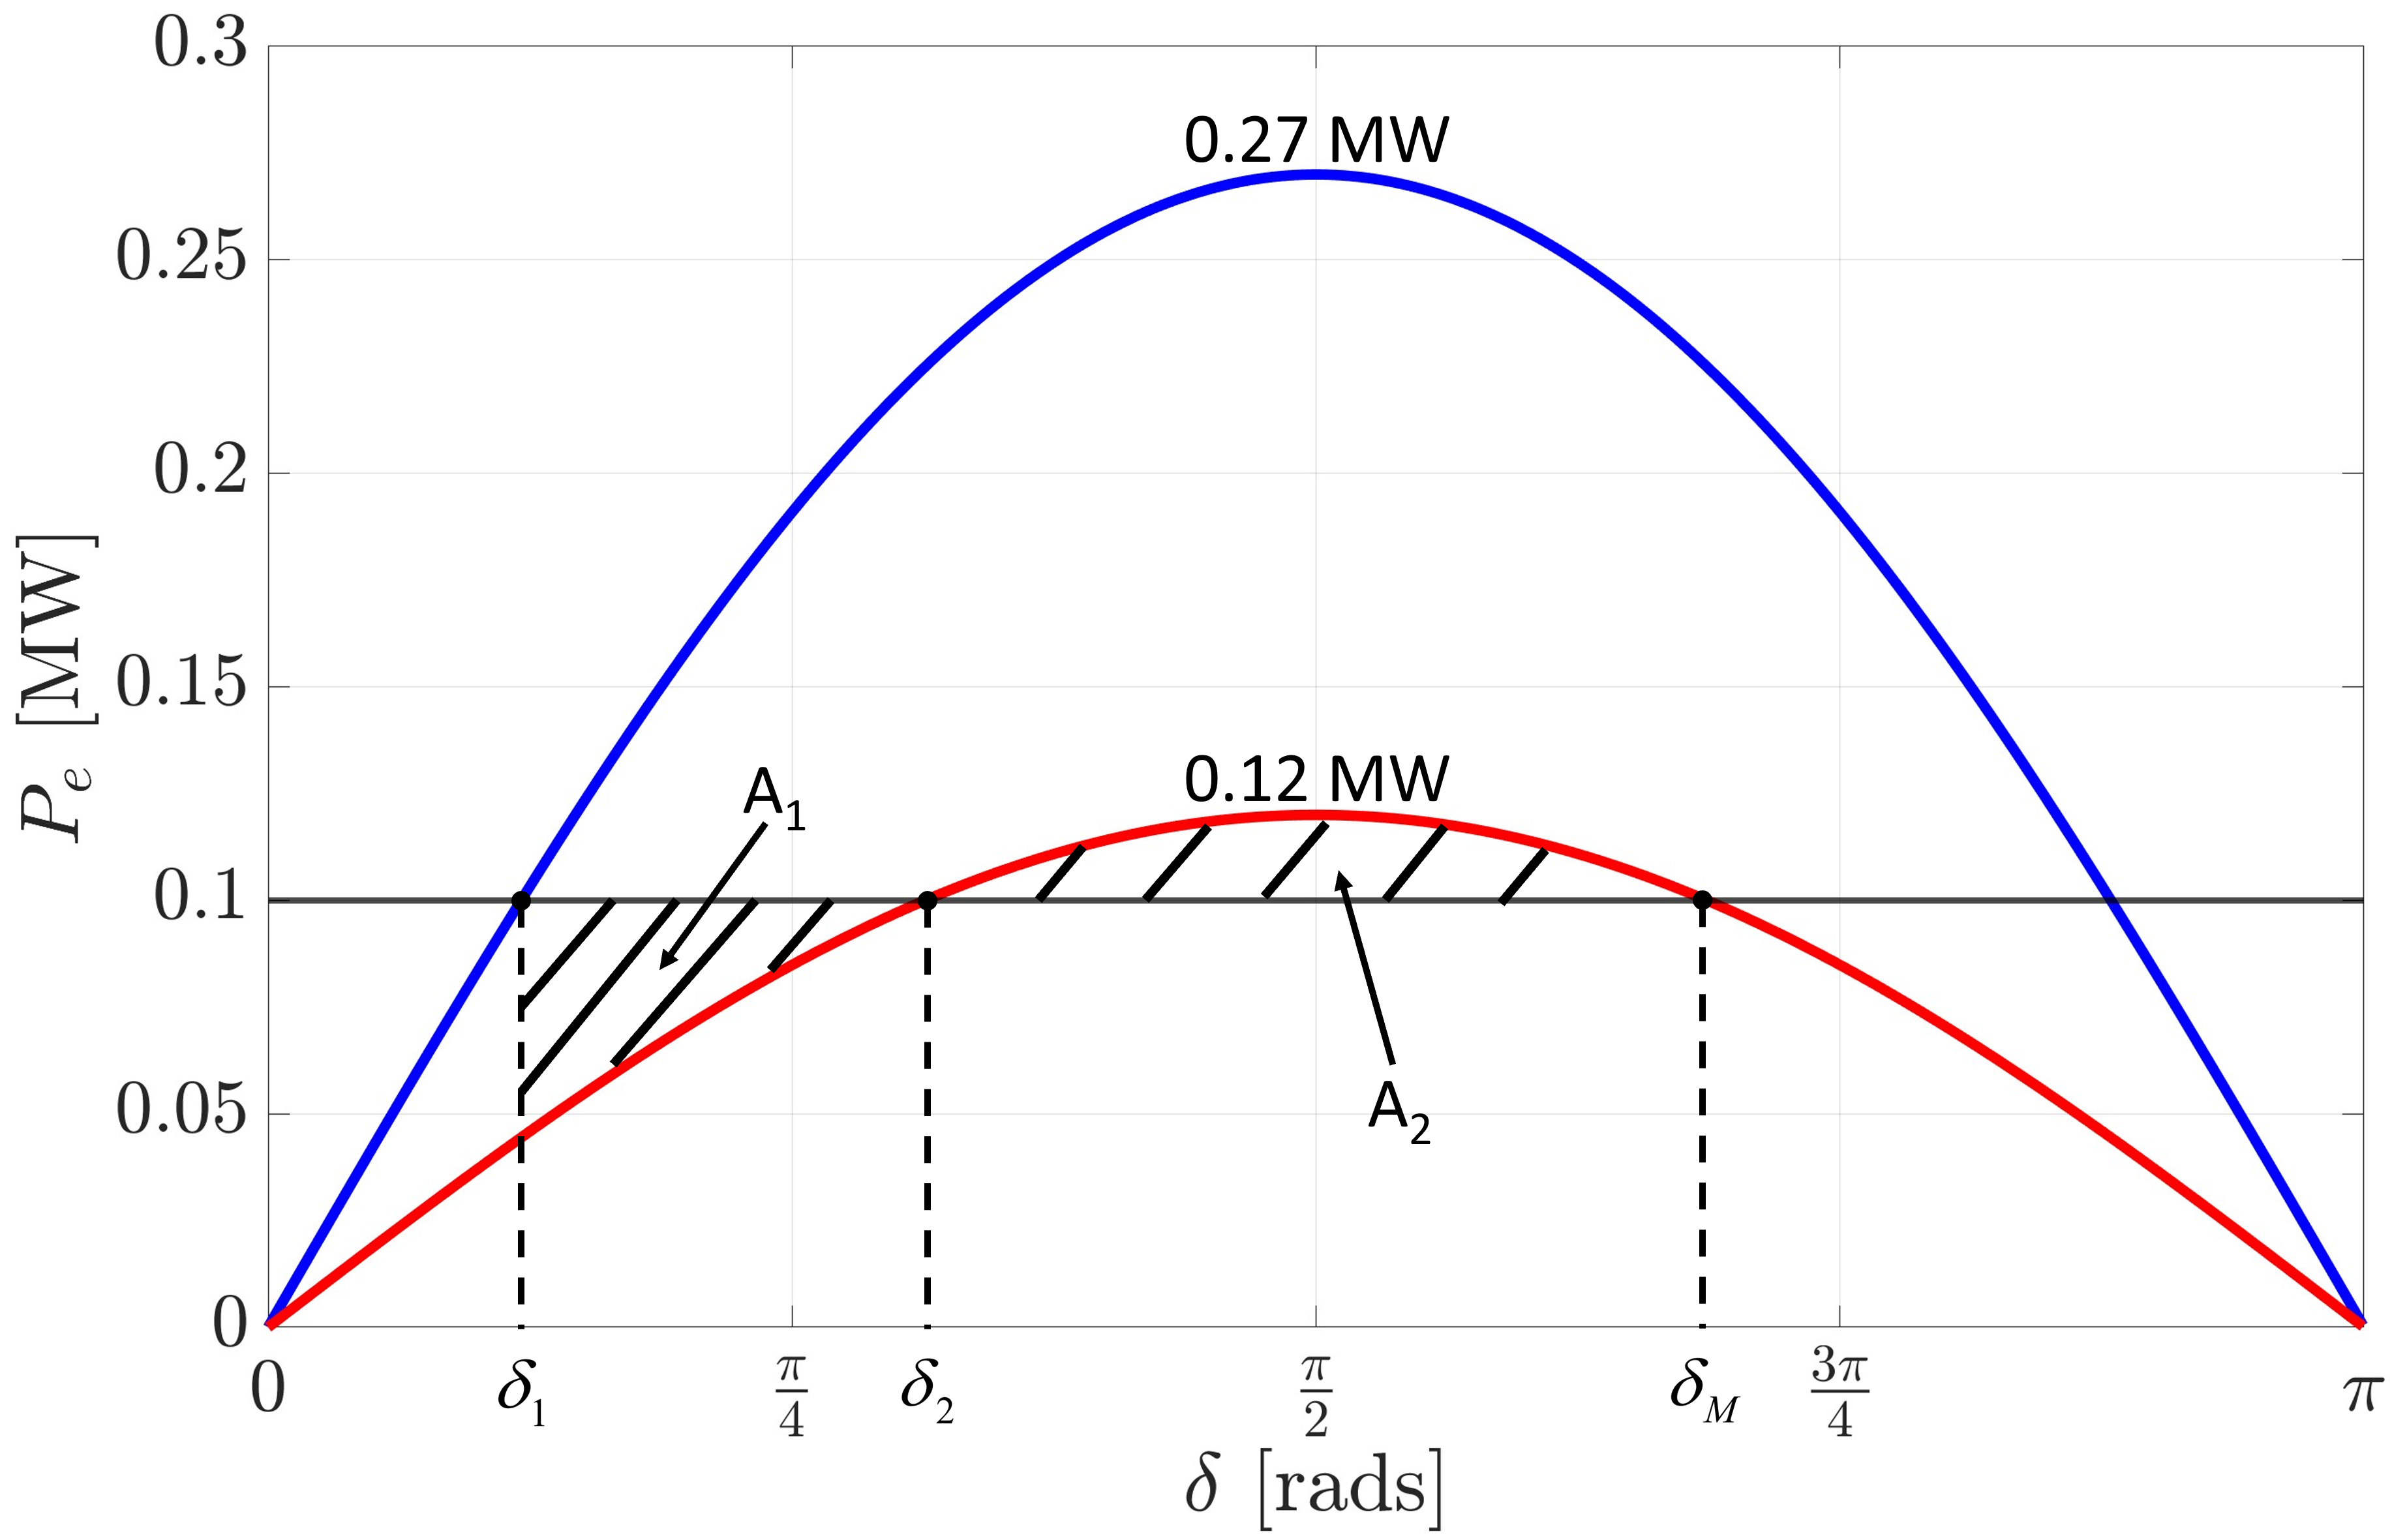
\includegraphics[width=\linewidth]{PEMDT Exam Report/img/12OnlyLine.png}
                 \caption{0.15 MW line fails so only 0.12 MW line remains in conduction}
                 \label{fig: 12onlyline}
            \end{subfigure}
            \hfill
            \begin{subfigure}{0.49\textwidth}
                 \centering
                 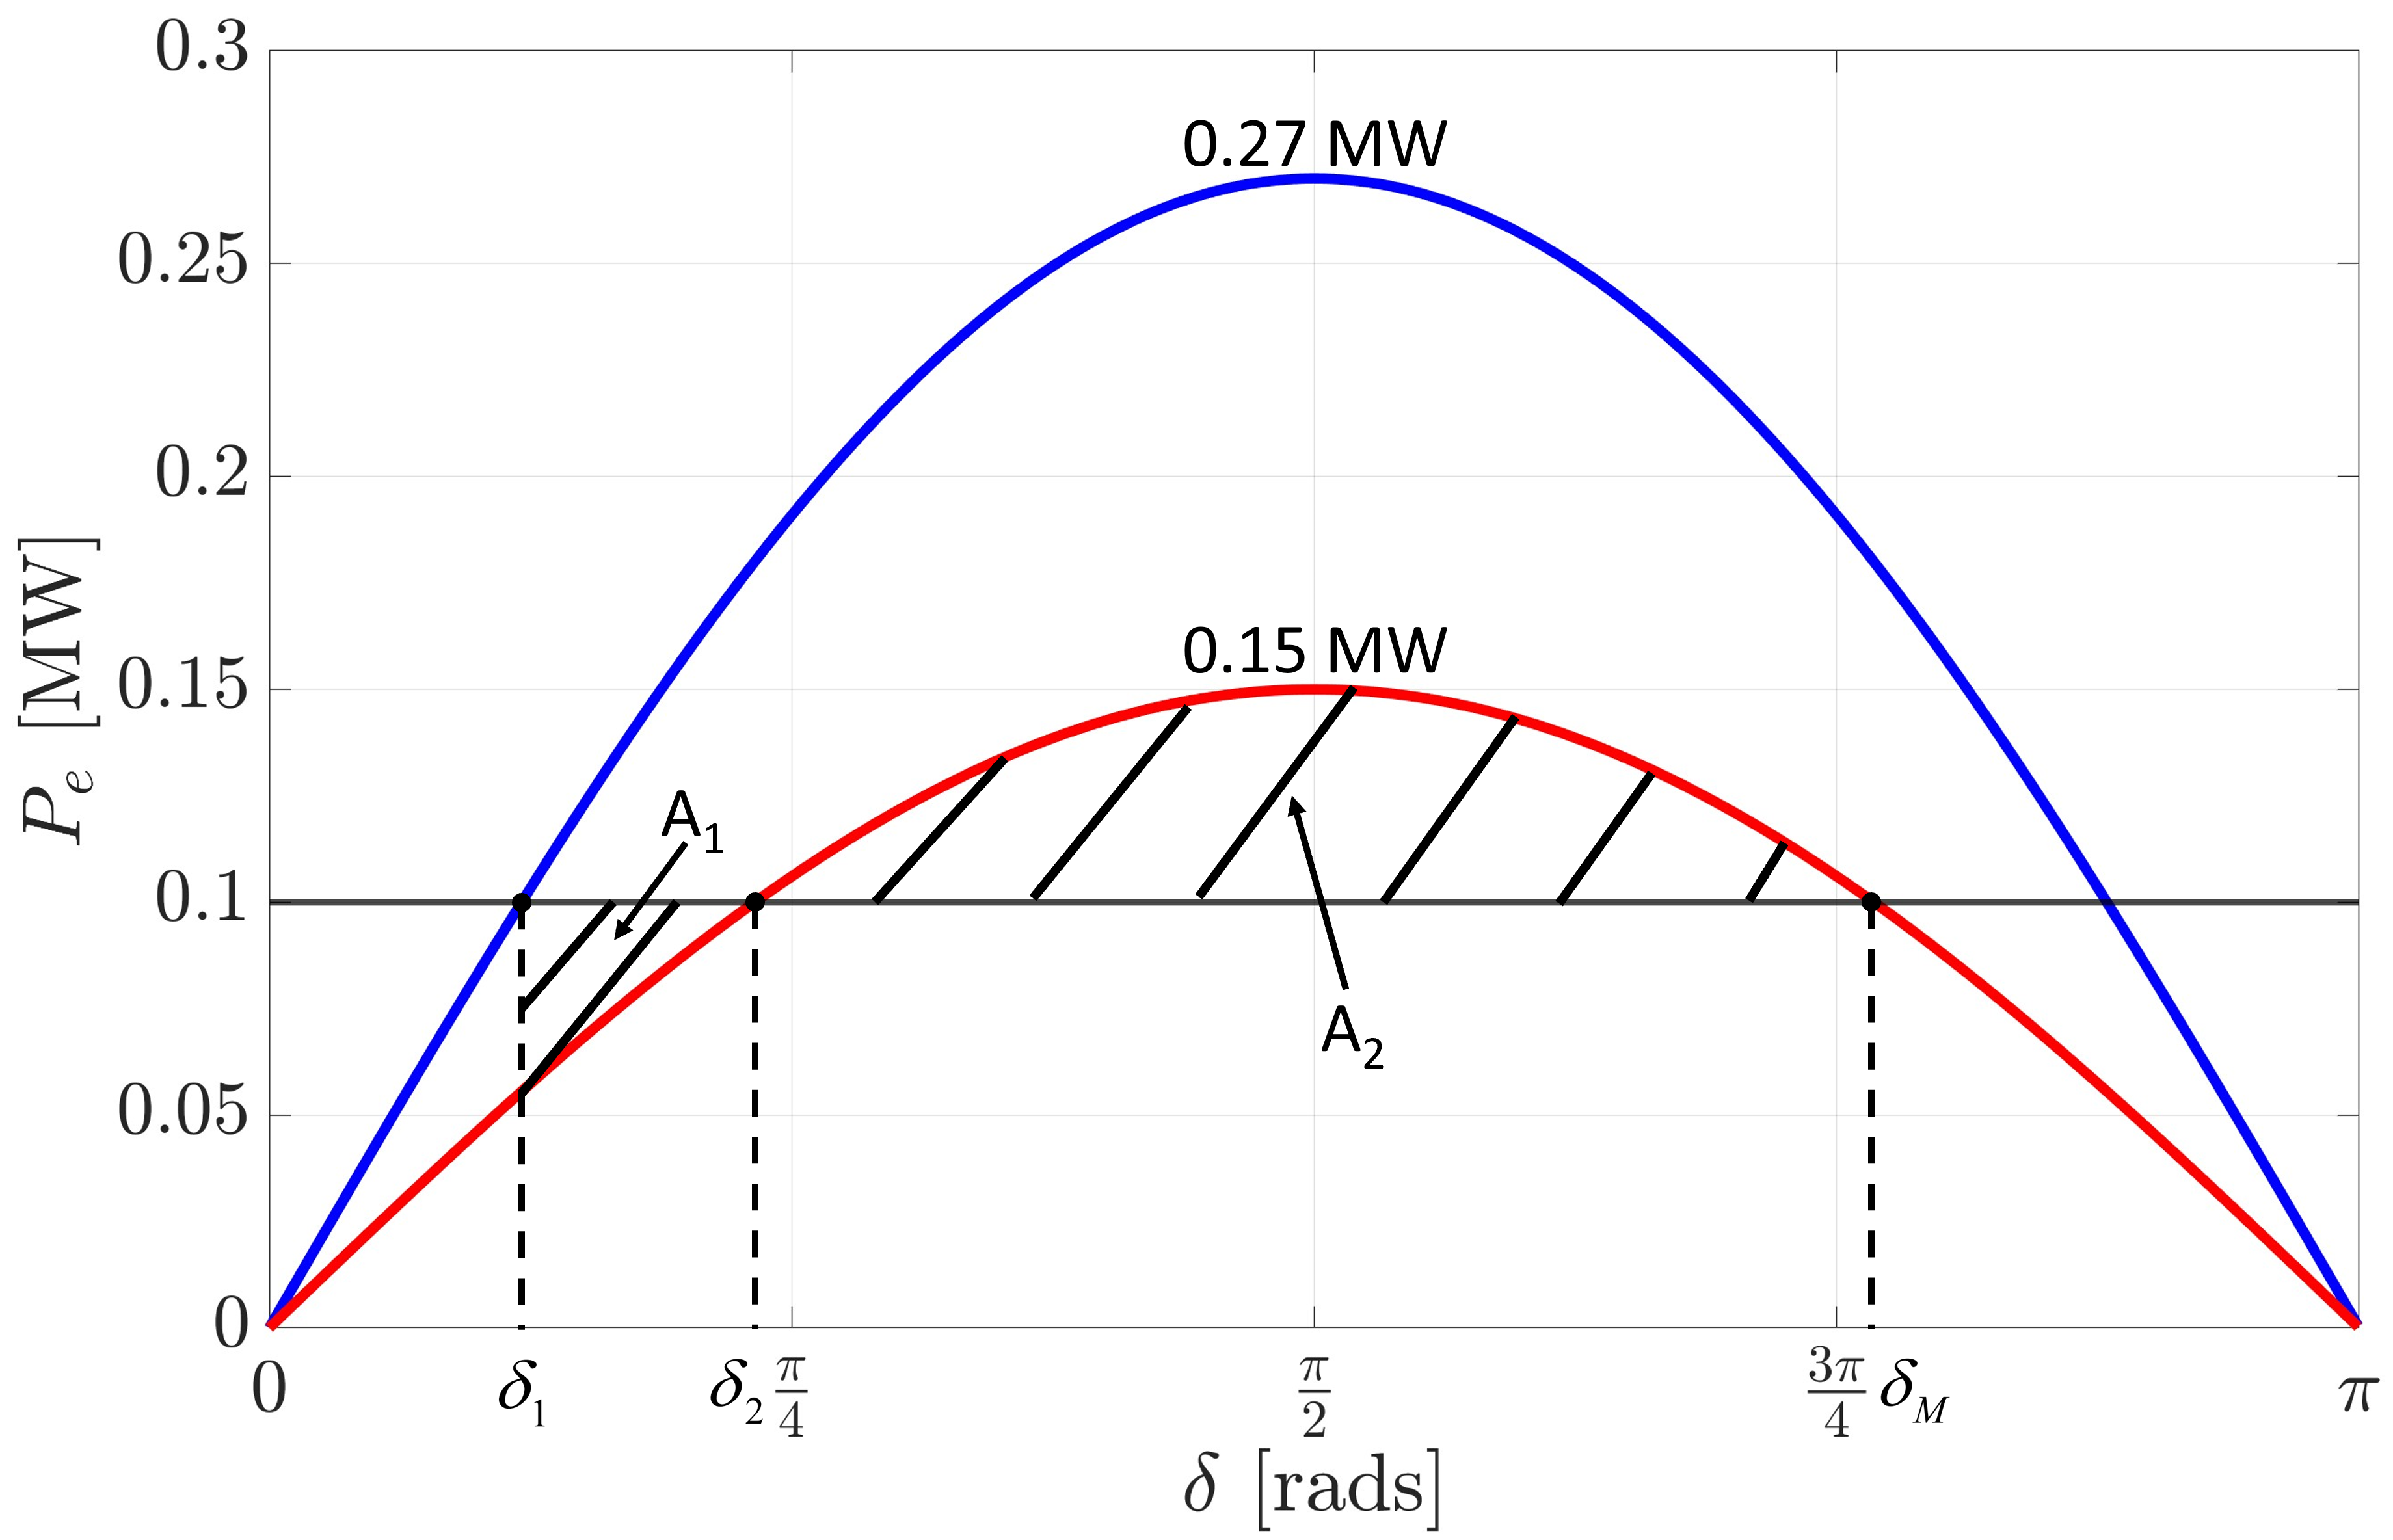
\includegraphics[width=\linewidth]{PEMDT Exam Report/img/15OnlyLine.png}
                 \caption{0.12 MW line fails so only 0.15 MW line remains in conduction}
                 \label{fig: 15onlyline}
             \end{subfigure}
             \caption{Power system stability if either a 0.12 MW line or 0.15 MW line fails after being in parallel with one another}
             \label{fig: line loss}
        \end{figure}
        \subsubsection*{0.15 MW Line Fails}
            When the 0.15 MW line fails, only the 0.12 MW line remains, as shown in Figure \ref{fig: 12onlyline}. To determine whether the system will stay in synchronisation Area \(A_2 \geq\) Area \(A_1\). 
    
            \begin{align}
                \delta_1 = sin^{-1}\left(\frac{0.1}{0.27}\right) = 0.379... && \delta_2 = sin^{-1}\left(\frac{0.1}{0.12}\right) = 0.985...\\
                A_1 = \int_{\delta_1}^{\delta_2}{0.1 - 0.12sin(\delta) \: d\delta} = 0.0154 && A_2 = 2\int_{\delta_2}^{\frac{\pi}{2}}{0.12sin(\delta) - 0.1 \: d\delta} = 0.0155
            \end{align}

            \(A_2 \geq A_1\); therefore, the system will stay in synchronisation under this fault.

        \subsubsection*{0.12 MW Line Fails}
            When the 0.12 MW line fails, only the 0.15 MW line remains, as shown in Figure \ref{fig: 15onlyline}. Once again, a similar comparison for the system under this failure is done to determine whether it stays in synchronisation. 
    
            \begin{align}
                \delta_1 = sin^{-1}\left(\frac{0.1}{0.27}\right) = 0.379... && \delta_2 = sin^{-1}\left(\frac{0.1}{0.15}\right) = 0.729...\\
                A_1 = \int_{\delta_1}^{\delta_2}{0.1 - 0.12sin(\delta) \: d\delta} = 0.00750 && A_2 = 2\int_{\delta_2}^{\frac{\pi}{2}}{0.12sin(\delta) - 0.1 \: d\delta} = 0.0554
            \end{align}

            \(A_2 \geq A_1\); therefore, the system will stay in synchronisation under this fault.

        \subsubsection*{Recommendations}
            \hl{Need to write any recommendations of how to ensure power systems remain stable}

    \subsection{}
        If the current (\(I_{a, b, c}\)) in a 3-phase system is unbalanced the positive (\(I_1\)), negative (\(I_2\)) and zero (\(I_0\)) sequences can be calculated using the following equations:
        \begin{align}
            I_{a1} = \frac{1}{3}\left(I_a + aI_b + a^2I_c\right) && I_{a2} = \frac{1}{3}\left(I_a + a^2I_b + aI_c\right) && I_{a0} = \frac{1}{3}\left(I_a + I_b + I_c\right), \label{sequence eqns}
        \end{align}
        where:
        \begin{align}
            I_a = 20\phase{15^o} = 20cos(15) + \textbf{j}20sin(15) \\
            I_b = 24\phase{-120^o} = 24cos(-120) + \textbf{j}24sin(-120) \\
            I_a = 18\phase{165^o} = 18cos(165) + \textbf{j}18sin(165)
        \end{align}
        \begin{align}
            a = 1\phase{-120^o} = -\frac{1}{2} + \textbf{j}\frac{\sqrt{3}}{2} && a^2 = 1\phase{-240^o} = -\frac{1}{2} - \textbf{j}\frac{\sqrt{3}}{2}
        \end{align}
        Substituting these values into Eq. (\ref{sequence eqns}), the following positive, negative and zero sequences were found for all 3 phases.
        \begin{align}
            I_{a1} &= 3.99 + \textbf{j}6.19 = 4.91\phase{35.60^o} \\ I_{b1} &= 0.48 - \textbf{j}4.87 = 4.91\phase{-84.40^o} \\
            I_{c1} &= -4.47 + \textbf{j}2.03 = 4.91\phase{-204.40^o} \\
            I_{a2} &= 18.68 + \textbf{j}5.97 = 19.61\phase{17.72^o} \\ I_{b2} &= -14.51 + \textbf{j}13.19 = 19.61\phase{137.72^o} \\
            I_{c2} &= -4.17 - \textbf{j}19.16 = 19.61\phase{257.72^o} \\
            I_{a0, b0, c0} &= -3.36 - \textbf{j}3.65 = 4.96\phase{-132.60^o}
        \end{align}
        \hl{Need to write how they can be used to detect faults}